\documentclass[border=4pt]{standalone}
% Shared by the independently buildable vector figures.
\usepackage[T1]{fontenc}
\usepackage{amsmath,amssymb,newpxtext,newpxmath}
\usepackage[semibold]{sourcesans}
\usepackage{pgfplots}
\pgfplotsset{compat=1.18}
\usetikzlibrary{arrows.meta,calc,positioning}
\usepgfplotslibrary{groupplots}
\definecolor{ink}{HTML}{19303A}
\definecolor{sea}{HTML}{00675E}
\definecolor{clay}{HTML}{A24725}
\definecolor{muted}{HTML}{4C636C}
\definecolor{rulegray}{HTML}{CAD4D4}
\definecolor{wash}{HTML}{EAF4F0}
\definecolor{warm}{HTML}{F7EEE5}
\color{ink}
\tikzset{every picture/.style={font=\sffamily\small},
  arrow/.style={-{Stealth[length=2mm]},line width=.8pt,draw=muted}}
\pgfplotsset{companion/.style={axis lines=left,axis line style={draw=muted},
  tick style={draw=muted},ticklabel style={font=\sffamily\footnotesize,text=muted},
  label style={font=\sffamily\small},grid=major,grid style={draw=rulegray!64,line width=.25pt},
  tick align=outside,enlarge x limits=false,scaled ticks=false,
  every axis plot/.append style={line join=round},
  legend style={draw=none,fill=none,font=\sffamily\footnotesize},
  title style={font=\sffamily\bfseries\small,anchor=south west,at={(0,1.03)}}}}

\begin{document}
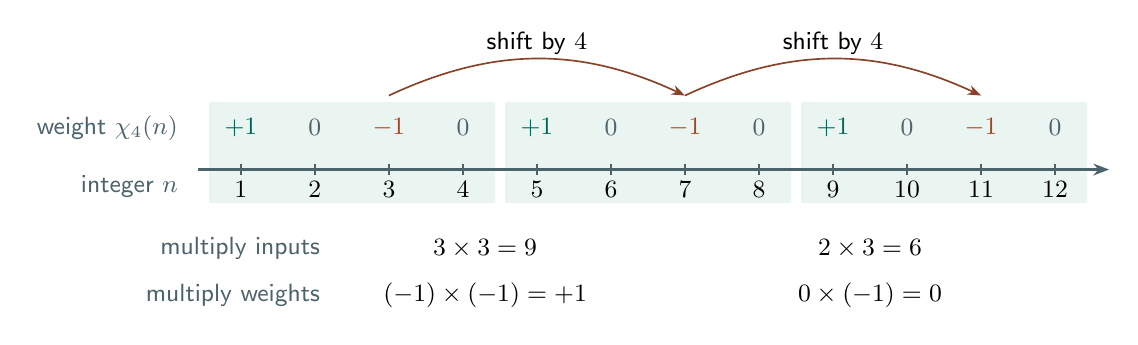
\begin{tikzpicture}[x=.94cm,y=1cm]
% Align each character value with its integer on the axis.
\foreach \start in {1,5,9}{
  \fill[wash] ({\start-.43},-.43) rectangle ({\start+3.43},.86);
}
\draw[arrow] (.42,0)--(12.73,0);
\node[anchor=east,text=muted] at (.28,.52) {weight $\chi_4(n)$};
\node[anchor=east,text=muted] at (.28,-.21) {integer $n$};
\foreach \start in {1,5,9}{
  \foreach \j/\weight/\tone in {0/+1/sea,1/0/muted,2/-1/clay,3/0/muted}{
    \pgfmathtruncatemacro{\integer}{\start+\j}
    \draw[muted,line width=.55pt] (\integer,-.065)--(\integer,.065);
    \node at (\integer,-.25) {$\integer$};
    \node[text=\tone] at (\integer,.53) {$\weight$};
  }
}
\foreach \a/\b in {3/7,7/11}{
  \draw[-{Stealth[length=1.7mm]},draw=clay!80!ink,line width=.6pt]
    (\a,.94) to[out=25,in=155] node[midway,above,inner sep=1.5pt] {shift by $4$} (\b,.94);
}

\node[anchor=east,text=muted] at (2.2,-1.00) {multiply inputs};
\node[anchor=east,text=muted] at (2.2,-1.60) {multiply weights};
\foreach \x/\leftin/\rightin/\product/\leftwt/\rightwt/\outwt in {
  4.3/3/3/9/{(-1)}/{(-1)}/{+1},
  9.5/2/3/6/0/{(-1)}/0}{
  \node at (\x,-1.00) {$\leftin\times\rightin=\product$};
  \node at (\x,-1.60) {$\leftwt\times\rightwt=\outwt$};
}
\end{tikzpicture}
\end{document}
